\section{Background and the key kernels}
\todo[inline, color=red!40]{This work use custom processing elements to accelerate the compute intensive pair-hmm alignment step.}

\subsection{Second and Third Generation Reads}
\textbf{GATK Pipeline.}~xxx this is the time consuming motivation. Second, many kernels are invoked many times in the whole pipeline.

\subsection{Variant Calling in the pipeline}
\textbf{Variant Calling Steps.}~As shown in Fig.~\ref{}, 

\begin{figure}[htbp]
\centering
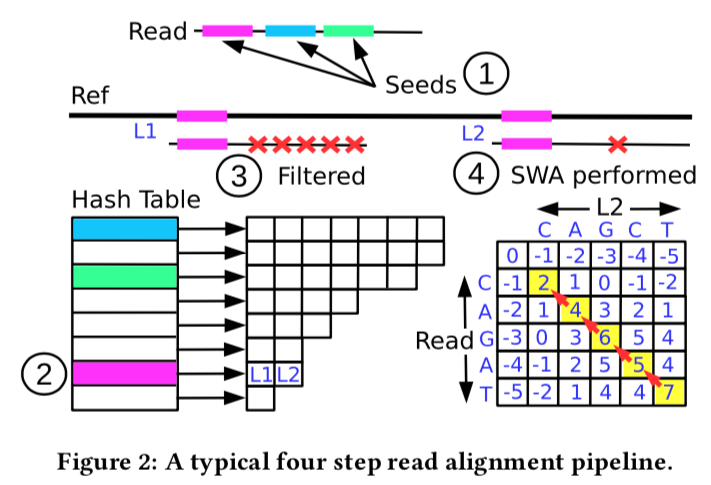
\includegraphics[scale=0.32]{fig/demo-steps.png}
\caption{A typical four step variant calling pipeline}
\label{fig:arch_design}
\end{figure}

\subsection{Variant calling algorithms}
Even though variant calling algorithms have been evolving and recently more and more algorithms have moved from position-based (\textit{e.g.} Mutect1~\cite{}) to graph-base (\textit{e.g.} HaplotypeCaller, Mutect2~\cite{}), and DNN-based algorithms (\textit{e.g.} applied somatic DeepVariant~\cite{}), most non-position-based algorithms are still being improved. 

%to write the distribution of three major pipelines
\subsection{Pair-HMM Algorithm}
this
\subsubsection{Algorithm description}
As a variant of Smith-Waterman algorithm, Pair-HMM is commonly used in variant-calling. The hidden Markov model is used in Pair-HMM to generate a probability score for the alignment between candidate haplotypes (H) and read sequences (R). Similar to Smith-Waterman algorithm, for a pair of nucleotides, there are three possibilities for one pair of sequences, i.e., match, insertion, and deletion. The The key difference is that Pair-HMM uses floating point operations.

The Pair-HMM algorithm takes a list of $N$ reads and a list of $M$ candidate haplotypes as input and returns the probability that the data would explain each one of the candidate haplotypes. To calculate the probability, the Pair-HMM performs assesses all possible alignments of each haplotype (the hypothesis) against all the reads (the data). The HMM has three main states: match, insertion and deletion. Here we introduce three concepts related to the base quality score ($Q_m$): The insertion gap open penalty (or base insertion quality $Q_i$), the deletion gap open penalty (or base deletion quality $Q_d$) and the gap continuation penalty ($Q_g$). The first two represent the probability that the base precedes an insertion or a deletion (respectively) and even when not reported by the instrument can be generated by the latest version of the Base Quality Score Recalibration tool (BaseRecalibrator) in the GATK [cite GATK]. The third represents the probability that an insertion or deletion are extended which in theory could be different for insertions and deletions, but in our model we use the same flat value $Q10$ for all gap continuation penalties.

\begin{figure}[htbp]
\centering
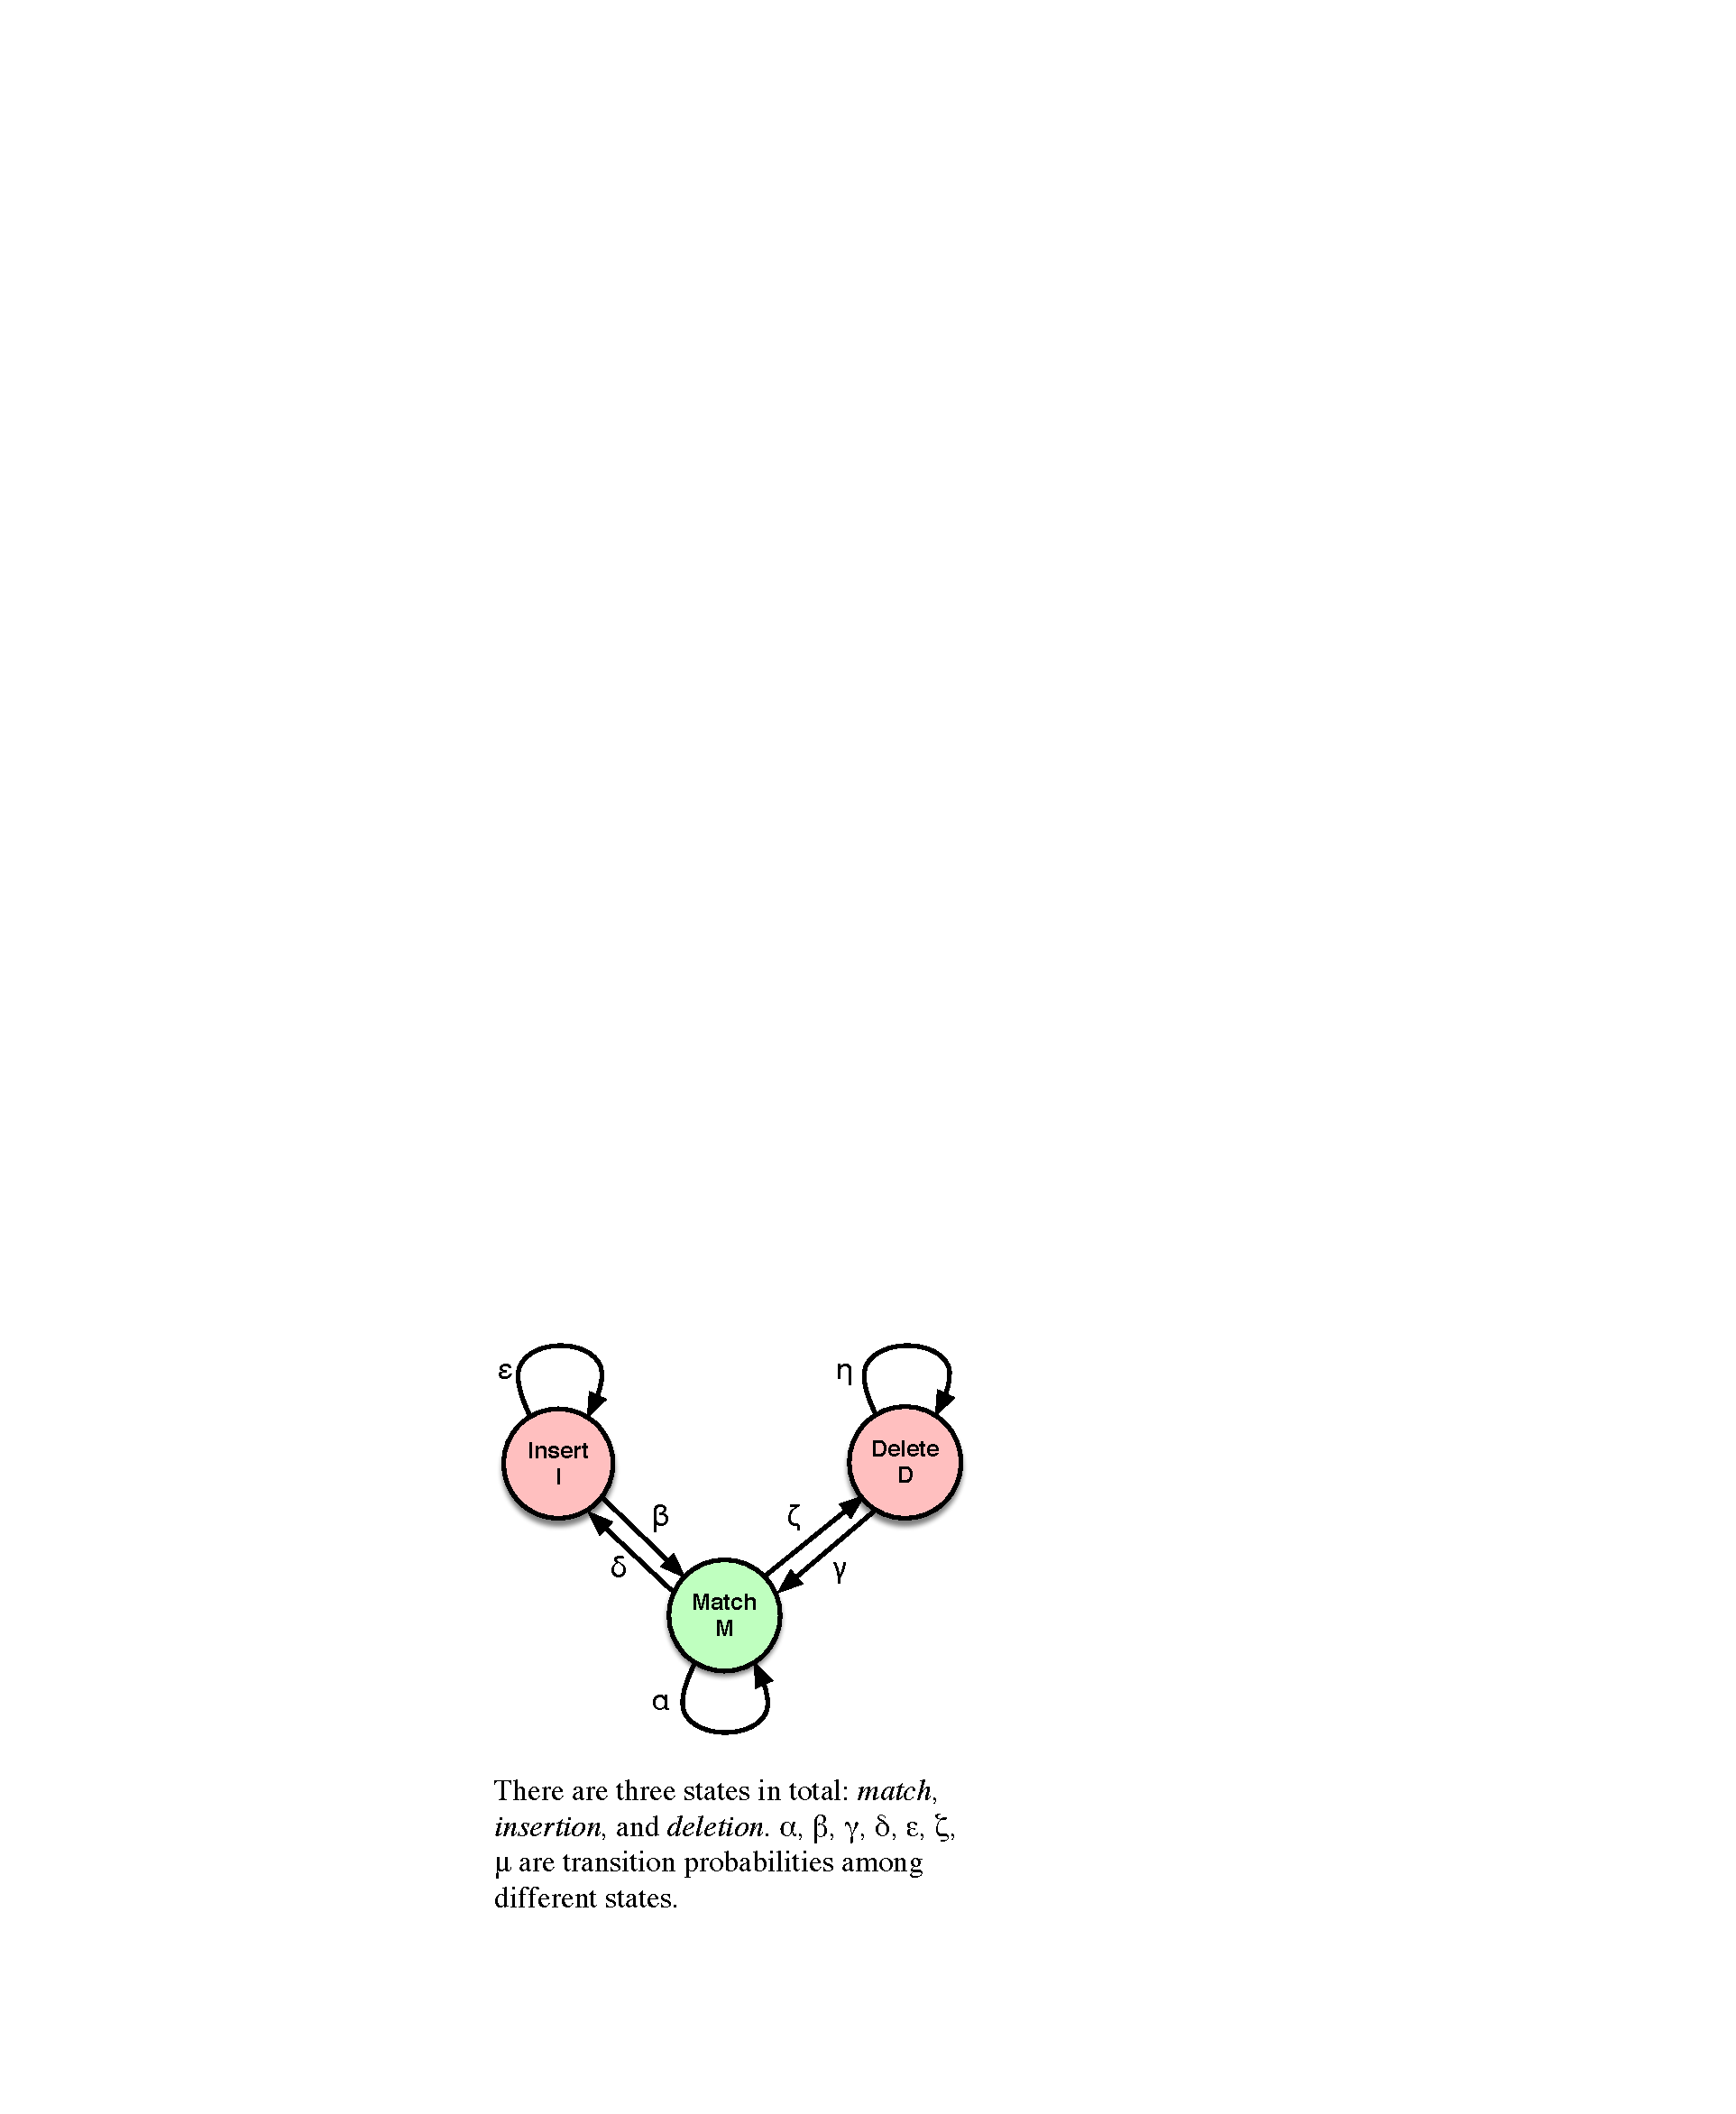
\includegraphics[scale=0.52]{fig/algo-pair-hmm.pdf}
\caption{Insert, delete, and match states of Pair-HMM.}
\label{fig:arch_design}
\end{figure}

The Pair-HMM accuracy relies on the accurate estimation of these four quality scores for every base. The Pair-HMM equations are described below:

\begin{align}
    M_{i,j} &= P_{i,j} (\alpha  M_{i-1,j-1} + \beta  I_{i-1,j-1} + \gamma D_{i-1,j-1} ) \\
    I_{i,j} &= \delta  M_{i-1,j} + \epsilon  I_{i-1,j} \\
    D_{i,j} &= \zeta   M_{i,j-1} + \eta  D_{i,j-1} 
\end{align}

Given that $Q_m$ is the base quality score of a base in the read converted from phred-scale to probability space using the formula $Q = -log_{10}P$. The prior $P_{i,j}$ is $1-Q_m$ of the $i^{th}$ base in the read if it matches the $j^{th}$ base in the haplotype, or $Q_m$ if it does not.  The transition probabilities are expressed by the roman letters in the equation and are described below: 

\begin{align*}
    \alpha   &= 1 - (Q_i + Q_d) \text{ | match continuation} \\
    \beta    &= 1 - Q_g \text{ | insertion to match} \\
    \gamma   &= 1 - Q_g \text{ | deletion to match} \\
    \delta   &= Q_i \text{ | match to insertion} \\
    \epsilon &= Q_g \text{ | insertion continuation} \\
    \zeta    &= Q_d \text{ | match to deletion} \\
    \eta     &= Q_g \text{ | deletion continuation}
\end{align*}

The resulting probability is theoretically the sum of $M_{N,M}$, $I_{N,M}$ and $D_{N,M}$, however there are a two special conditions in this HMM that change:

\begin{enumerate}

\item To allow the alignment of the haplotype to start anywhere on the read without penalty, we need to initialize the entire first row of the deletion matrix with the normalized factor $\frac{1}{\text{len(}R_i\text{)}}$.

\item To allow the alignment to end anywhere in the read without penalty, we need to ignore the last row of the deletion matrix ($D$) in the final calculation of the Pair-HMM probability.

\end{enumerate}

The key difference is that Pair-HMM uses floating point operations. For this study, we used our optimized implementation that is also a part of the Genomics Kernel Library (GKL) by Intel.

\subsubsection{Inter- and Intra-parallelism}

\begin{figure}[htbp]
\centering
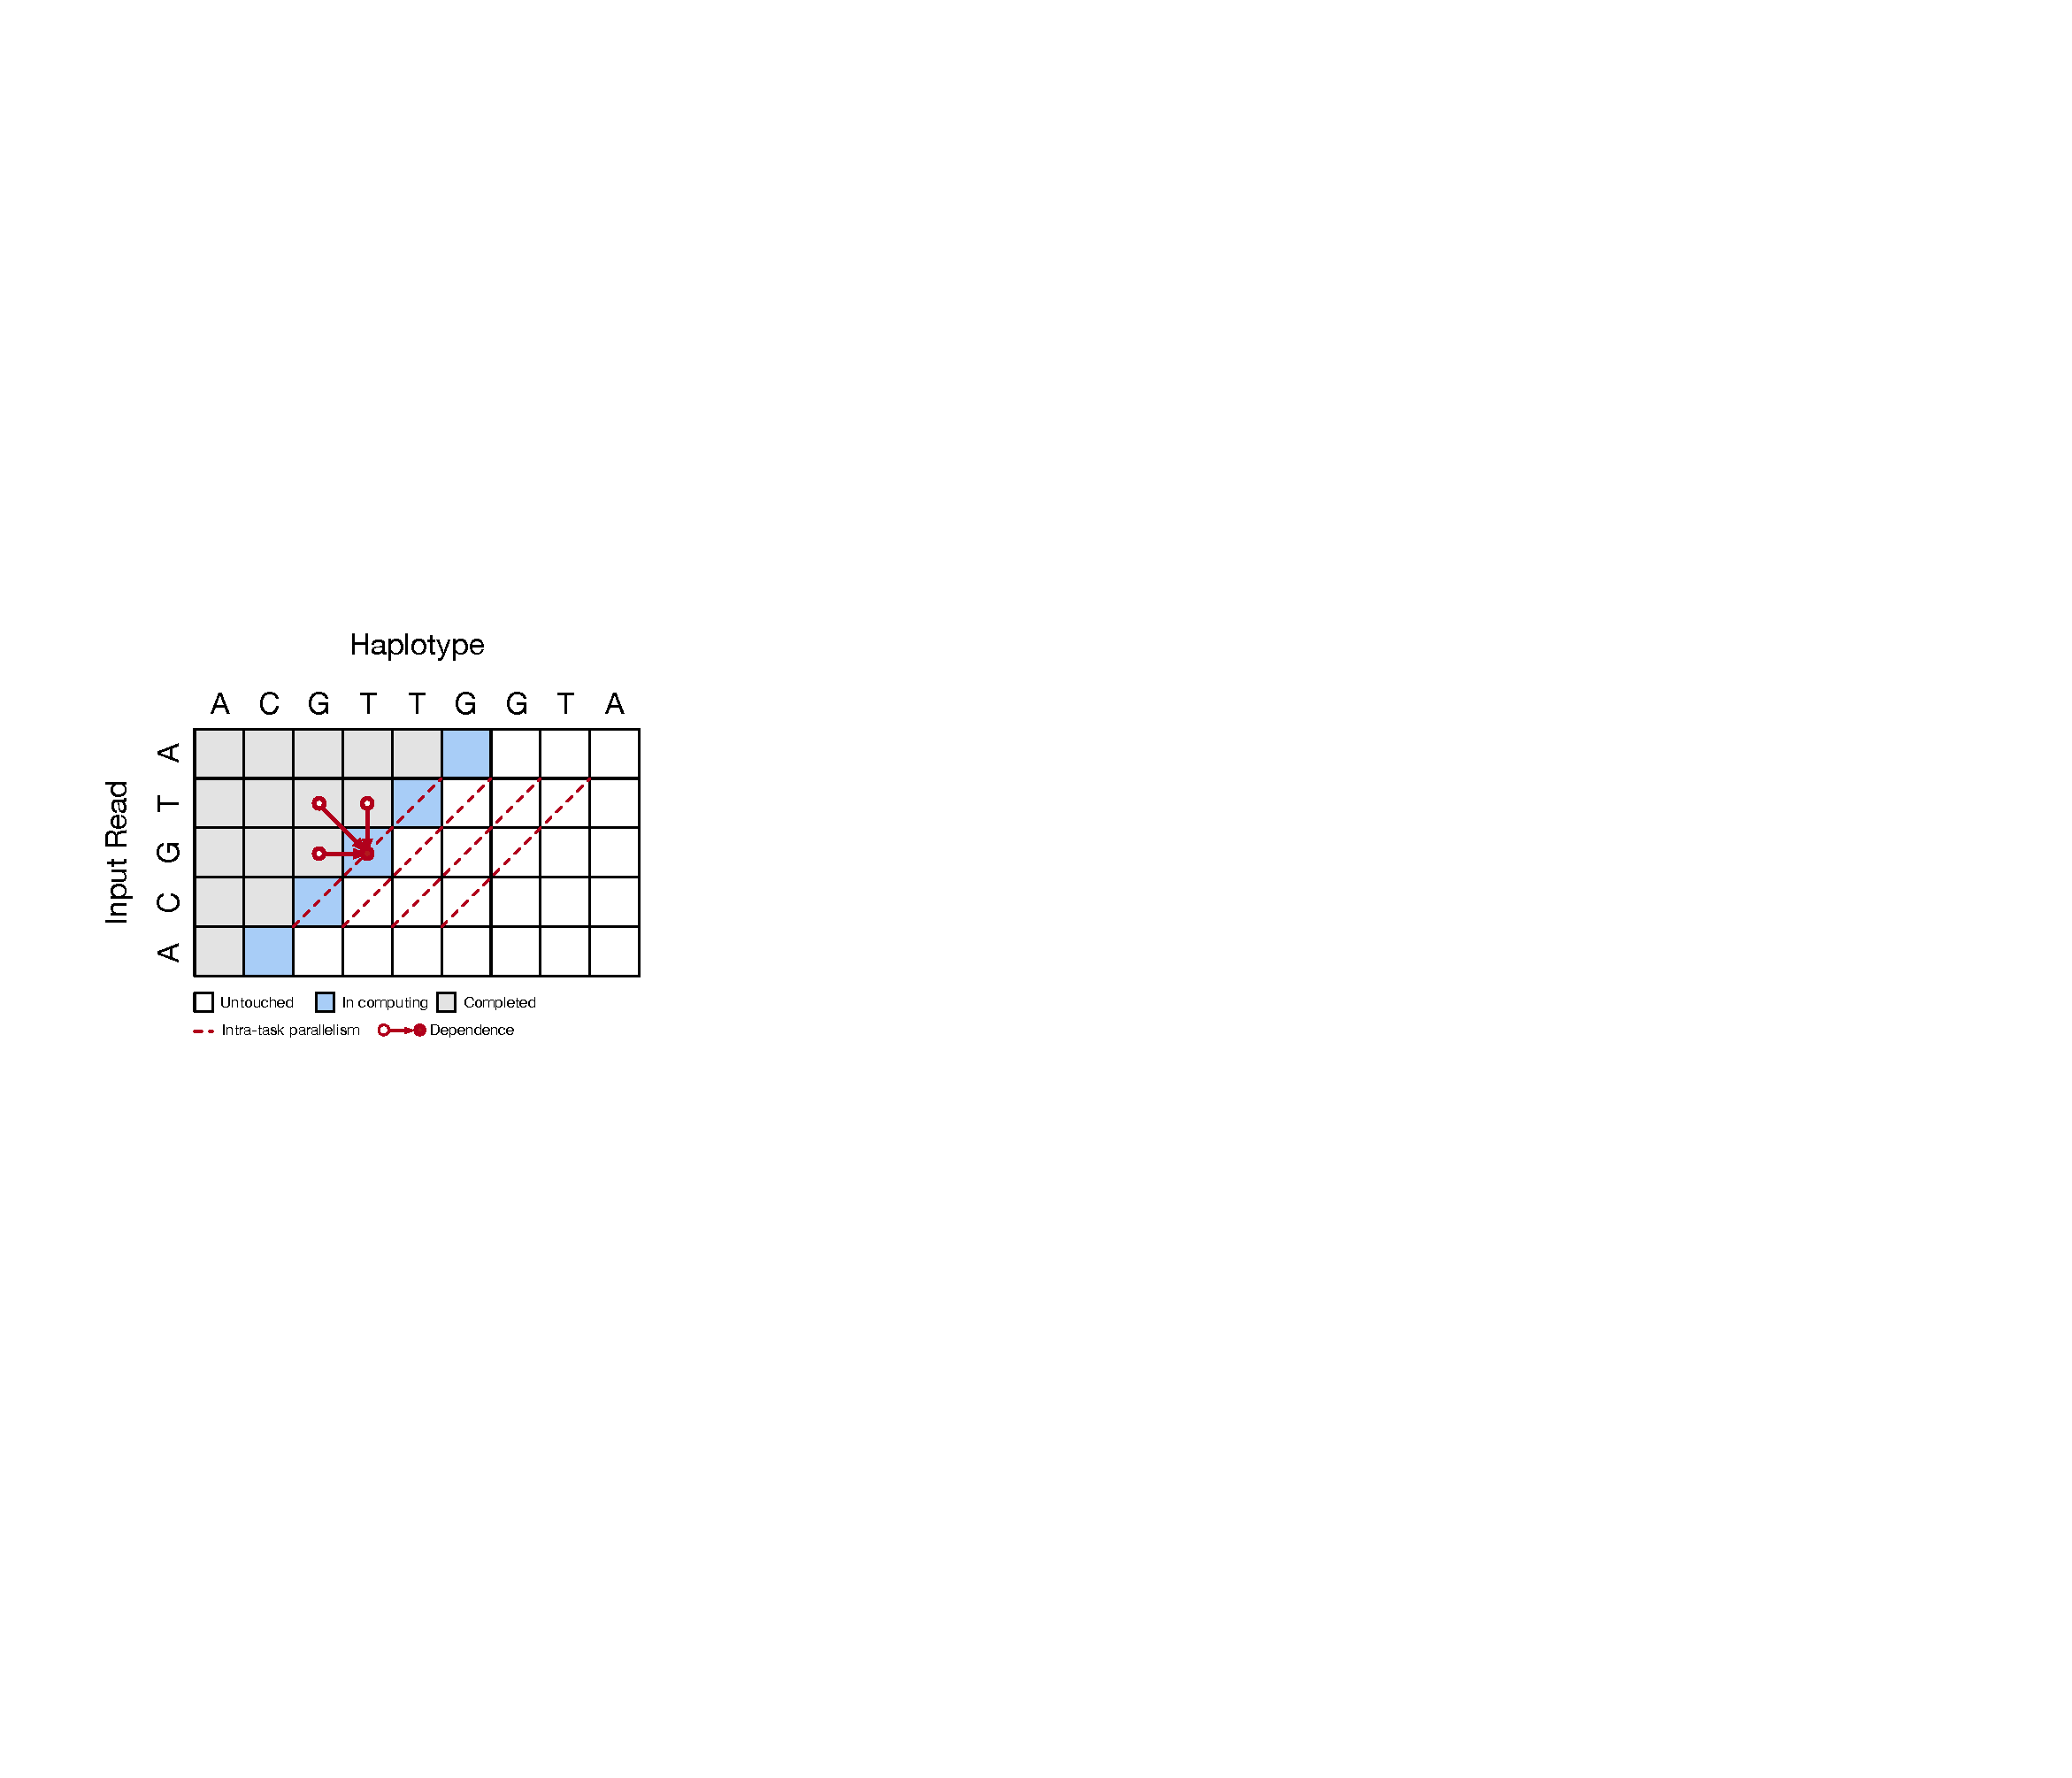
\includegraphics[width=\linewidth]{fig/algo-intra-parallelism.pdf}
\caption{}
\label{fig:para-pair-hmm}
\end{figure}


\subsection{Smith-Waterman}
